\documentclass[]{beamer}
% Class options include: notes, notesonly, handout, trans,
%                        hidesubsections, shadesubsections,
%                        inrow, blue, red, grey, brown
%\usepackage{caption}
\setbeamertemplate{caption}[numbered] 
\usepackage[absolute,overlay]{textpos}
\setlength{\TPHorizModule}{1mm} \setlength{\TPVertModule}{1mm}
\newcommand{\MyLogo}{%
\begin{textblock}{14}(115.9,0.1)
  
\includegraphics[width=1.22cm]{kth_rgb}
 \end{textblock}
}
\renewcommand{\raggedright}{\leftskip=0pt \rightskip=0pt plus 0cm}
\usepackage{sidecap}
% Theme for beamer presentation.
\usepackage{beamerthemesplit} 
\usepackage{amssymb}
\usepackage{theorem}
\usepackage{graphicx} % Include figure files
\usepackage{epstopdf}
\usepackage{amsmath} % Include the ast symbol
\usepackage{comment}  % Include the comment function
\usepackage[english]{babel}
\usepackage[latin1]{inputenc}
\usepackage{tikz}
\usetikzlibrary{shapes,arrows}
% Other themes include: beamerthemebars, beamerthemelined, 
%                       beamerthemetree, beamerthemetreebars  
\title{Parameterization of Energy Bands and Optical Properties in Semiconductor $CuIn_{1-x}Ga_{x}Se_2$}    % Enter your title between curly braces
\author{Rongzhen Chen}                % Enter your name between curly braces
\institute{{ {Multiscale Materials Modeling}}\\
           Department of Materials Science and Engineering \\
           {Royal Institute of Technology}}      % Enter your institute name between curly braces
\date{October 23, 2013}                    % Enter the date or \today between curly braces


\begin{document}

\MyLogo



% Creates title page of slide show using above information
\begin{frame}
  \titlepage
\MyLogo
\end{frame}
\note{Talk for 30 minutes} % Add notes to yourself that will be displayed when
                           % typeset with the notes or notesonly class options

\section[Outline]{}

\begin{frame}

 \tableofcontents

\MyLogo
\end{frame}


\section{Motivation}
\begin{frame}
\MyLogo
According to the statistical review of world energy on 2012. 
\begin{figure}[H]
     \begin{center}
            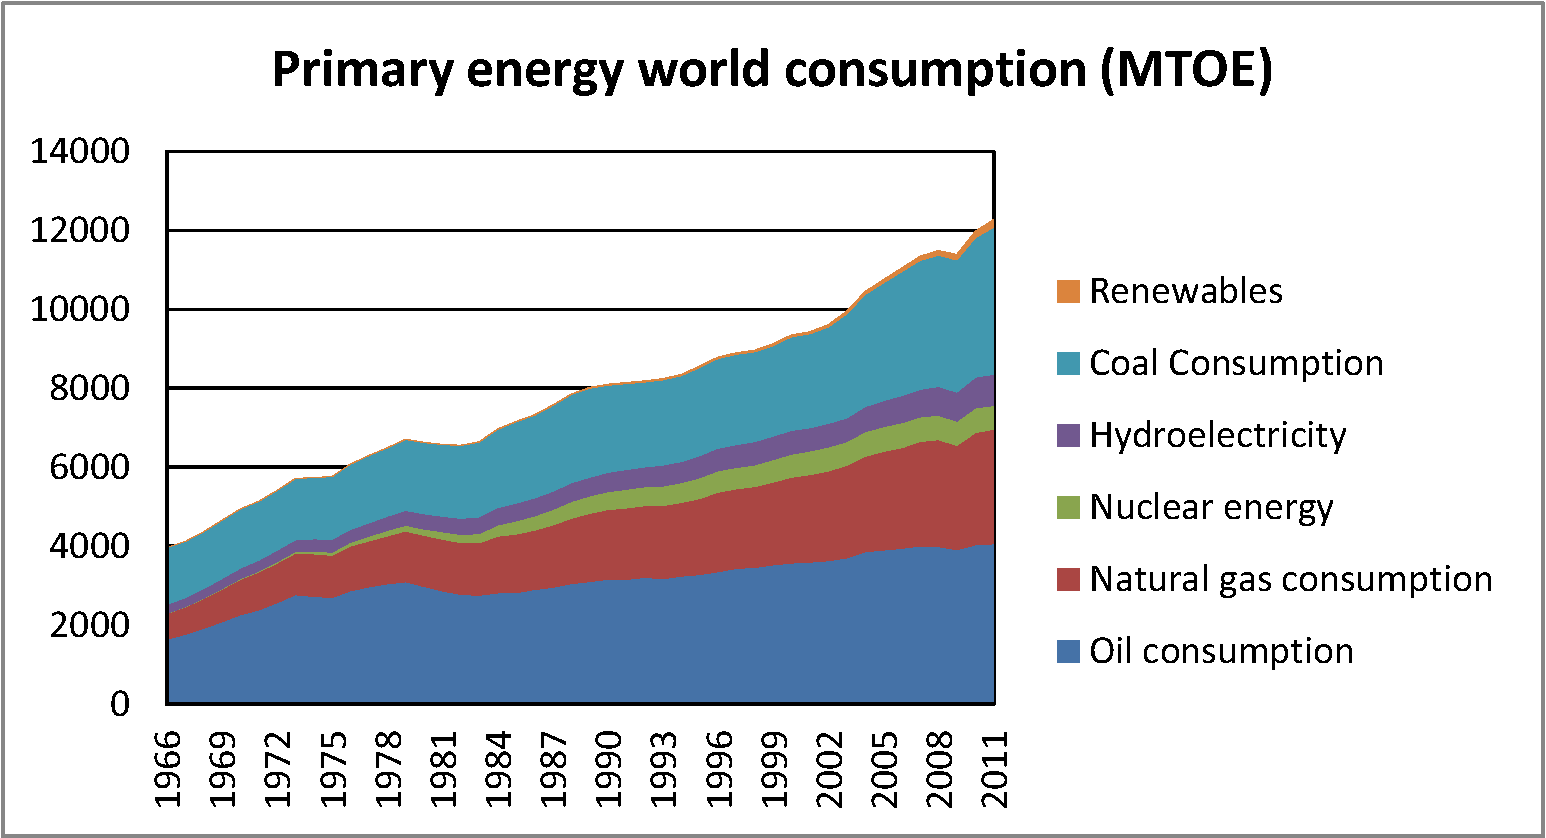
\includegraphics[width=0.8\textwidth]{world_Consumption.pdf}
     \end{center}
    \caption{ Figure is from BP statistical review of world energy 2012, METO means million tonnes oil equivalent. }
\end{figure}
\end{frame}

\begin{frame}
\MyLogo
\begin{figure}[H]
\centering
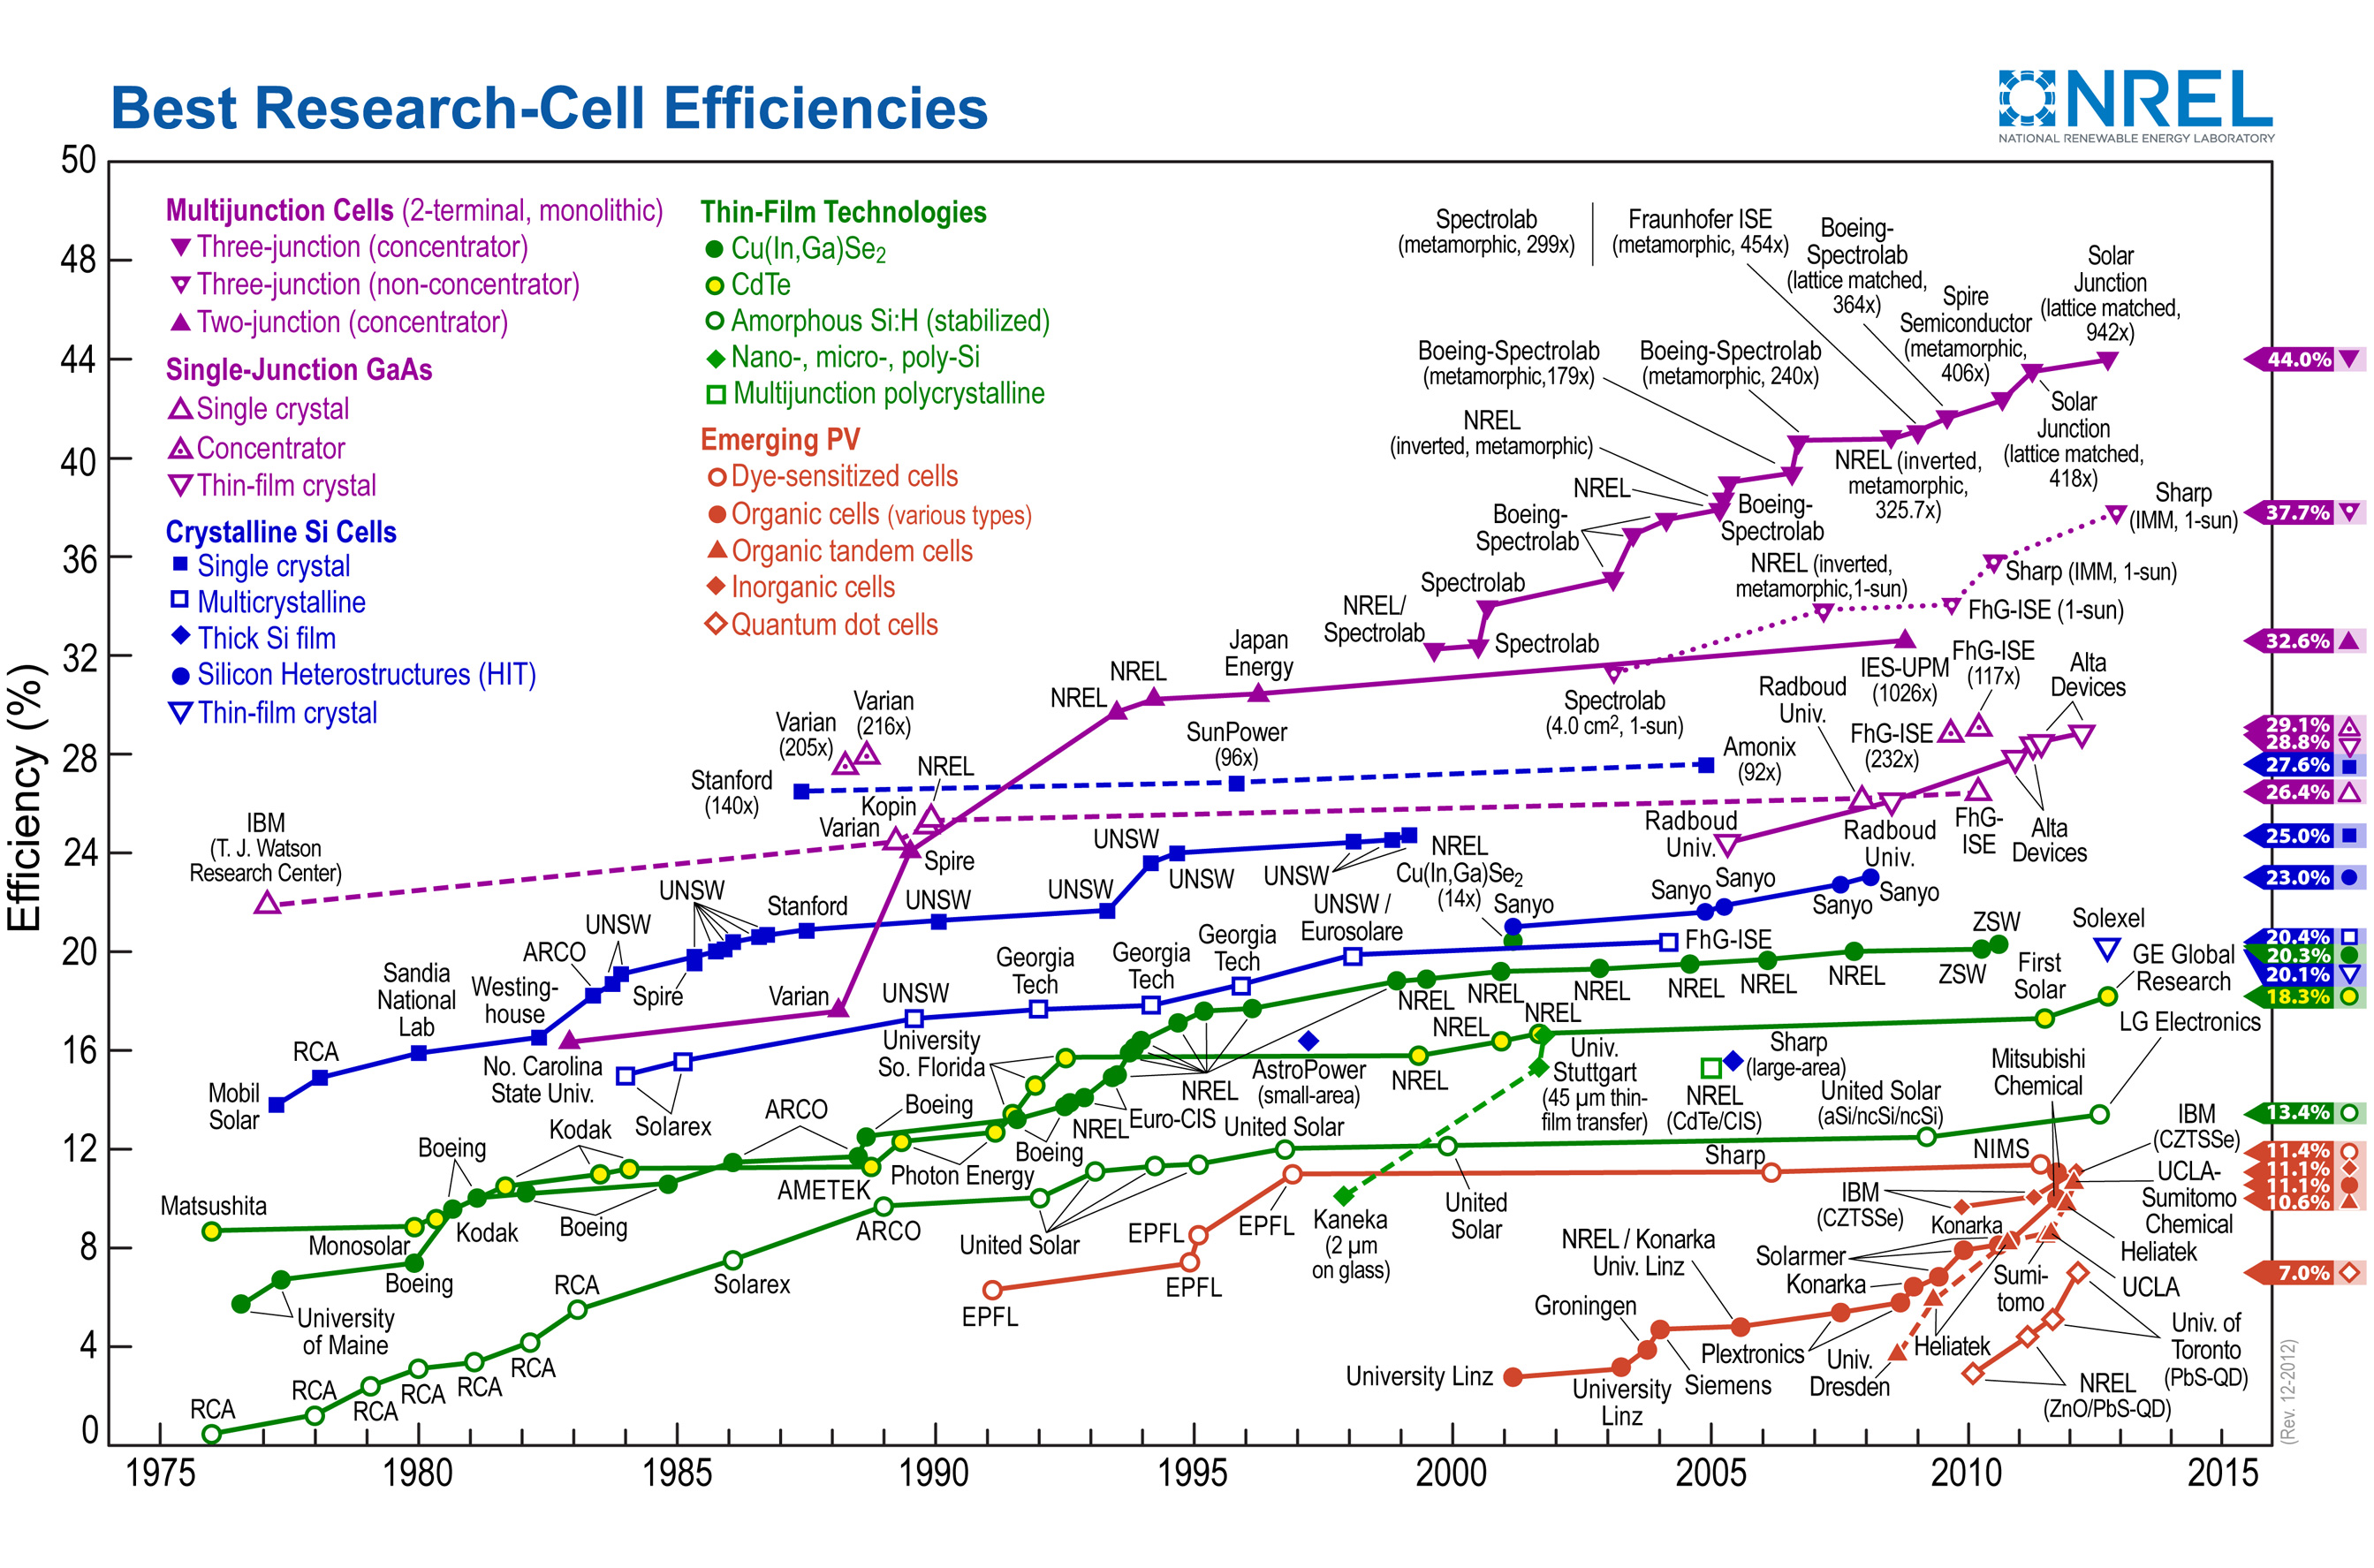
\includegraphics[width=0.8\textwidth]{efficiency_chart.jpg}
\caption{Best research-cell efficiencies. Figure is from National Renewable Energy Laboratory (NREL), Golden, Colorado.}
\label{nrel}
\end{figure}
\end{frame}

\begin{frame}
\MyLogo

\begin{figure}[H]
\centering
%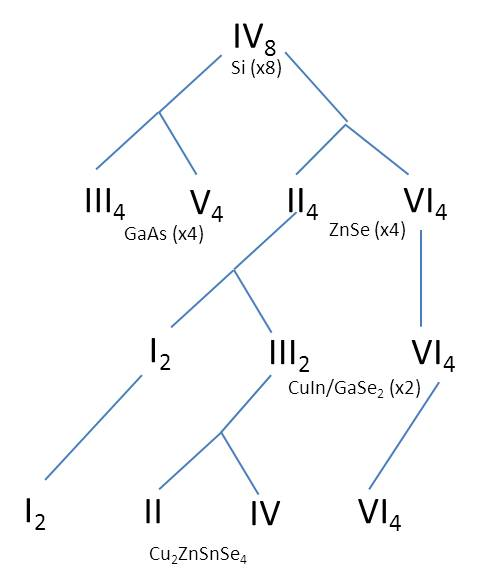
\includegraphics[scale=0.8]{compounds.jpg}
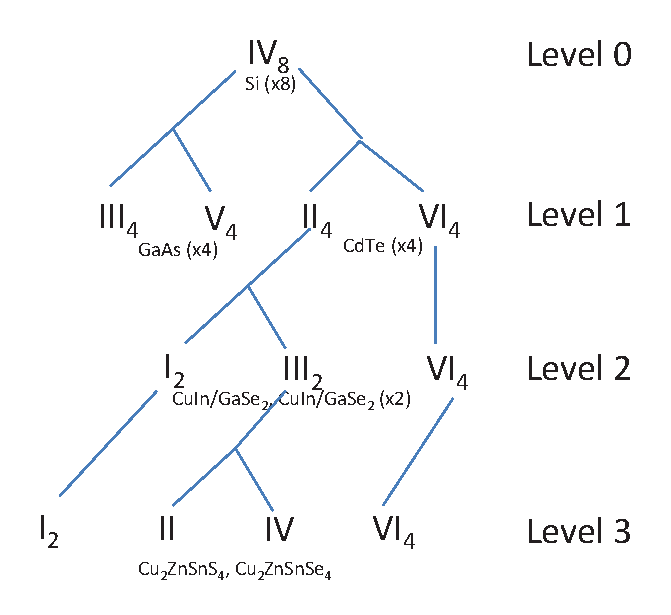
\includegraphics[width=0.5\textwidth,clip]{compoundsemicondctor1} 
\caption{Candidate of solar cell materials (absorption
coefficient, band gap range, cost and enviromental safety) .}
\label{compoundsemicondctor1}
\end{figure}
\end{frame}




\section{Parameterization of Energy Bands in $CuIn_{1-x}Ga_{x}Se_2$} 
\begin{frame}
\MyLogo

By considering the electron energy dispersion only around the $\Gamma$-point (centre of the Brillouin zone),
the parabolic band approximation (pba) is utilized:


\begin{equation}\label{parabolic}
E_{j}^{pb}(\textbf{k}) = E_{j}(\textbf{0}) \pm \left[ \frac{\widetilde{\textbf{k}}_{x}^{2}+\widetilde{ \textbf{k}}_{y}^{2}}{m_{j}^{\perp}} +  \frac{\widetilde{\textbf{k}}_{z}^{2}}{m_{j}^{\parallel}} \right]
\end{equation}


A common way to parameterize the energy bands is within the so called $K \cdot P$ approximation. However, 
the crystal-field interaction as well as the spin-orbit coupling of $CuIn_{1-x}Ga_{x}Se_2$ generates rather complex energy dispersions. 
So we extend the $K \cdot P$ expressions to higher orders.
\end{frame}

\begin{frame}
\MyLogo
\begin{equation}\footnotesize
\label{parabolic}\begin{split}
& \small E_j(\textbf{k}) = E_{j}^{pb}(\textbf{k}) + E_j^0 + \Delta_{j,1} \left( \delta_{j,1}^2 \left(  \frac{\widetilde{\textbf{k}}_{x}^{4}+\widetilde{ \textbf{k}}_{y}^{4}}{m_{0}^{2}} \right)  + \delta_{j,2}^2 \left( \frac{\widetilde{\textbf{k}}_{x}^{2}\widetilde{\textbf{k}}_{y}^{2}}{m_{0}^2}  \right) + 1 \right)^{1/2}  \\
& \small +  \Delta_{j,2} \left( \delta_{j,3}^3 \left(  \frac{\widetilde{\textbf{k}}_{x}^{6}+\widetilde{ \textbf{k}}_{y}^{6}}{m_{0}^{3}} \right)  + \delta_{j,4}^3 \left( \frac{\widetilde{\textbf{k}}_{x}^{2}\widetilde{\textbf{k}}_{y}^{4} + \widetilde{\textbf{k}}_{x}^{4}\widetilde{\textbf{k}}_{y}^{2}}{m_{0}^3}  \right) + 1 \right)^{1/3}  \\
& \small +  \Delta_{j,3} \left( \delta_{j,5}^2 \left(  \frac{\widetilde{\textbf{k}}_{z}^{4}}{m_0^2} \right) + 1 \right)^{1/2} + \Delta_{j,4} \left( \delta_{j,6}^3 \left(  \frac{\widetilde{\textbf{k}}_{z}^{6}}{m_0^3} \right) + 1 \right)^{1/3} \\
& \small +  \Delta_{j,5} \left( \delta_{j,7}^2 \left( \frac{\widetilde{\textbf{k}}_{x}^{2}\widetilde{\textbf{k}}_{z}^{2} + \widetilde{\textbf{k}}_{y}^{2}\widetilde{\textbf{k}}_{z}^{2}}{m_{0}^3}  \right) + 1 \right)^{1/2} \\
& \small +  \Delta_{j,6} \left( \delta_{j,8}^3 \left( \frac{\widetilde{\textbf{k}}_{x}^{4}\widetilde{\textbf{k}}_{z}^{2} + \widetilde{\textbf{k}}_{y}^{4}\widetilde{\textbf{k}}_{z}^{2}}{m_{0}^3}  \right) + \delta_{j,9}^3 \left( \frac{\widetilde{\textbf{k}}_{x}^{2}\widetilde{\textbf{k}}_{z}^{4} + \widetilde{\textbf{k}}_{y}^{2}\widetilde{\textbf{k}}_{z}^{4}}{m_{0}^3}  \right) +  \delta_{j,10}^3 \left( \frac{\widetilde{\textbf{k}}_{x}^{2}\widetilde{\textbf{k}}_{y}^{2}\widetilde{\textbf{k}}_{z}^{2}}{m_{0}^3}  \right) +1 \right)^{1/3} 
\end{split}\end{equation}
\end{frame}


\begin{frame}
\MyLogo
Unfortunately, the rather complex VB energy dispersions of $CuIn_{1-x}Ga_{x}Se_2$ require quite many fitting parameters. The CB, however, needs less parameters.

\vspace*{3\baselineskip}

The lowest conduction band (CB) and the three uppermost valence bands (VBs) of $CuIn_{1-x}Ga_{x}Se_2$ (x=0, 0.5, and 1) in order to better describe of the non-parabolic and anisotropic.
\end{frame}


\begin{frame}
\MyLogo
\begin{figure}\label{bandstr}
  \begin{minipage}{0.5\textwidth} 
    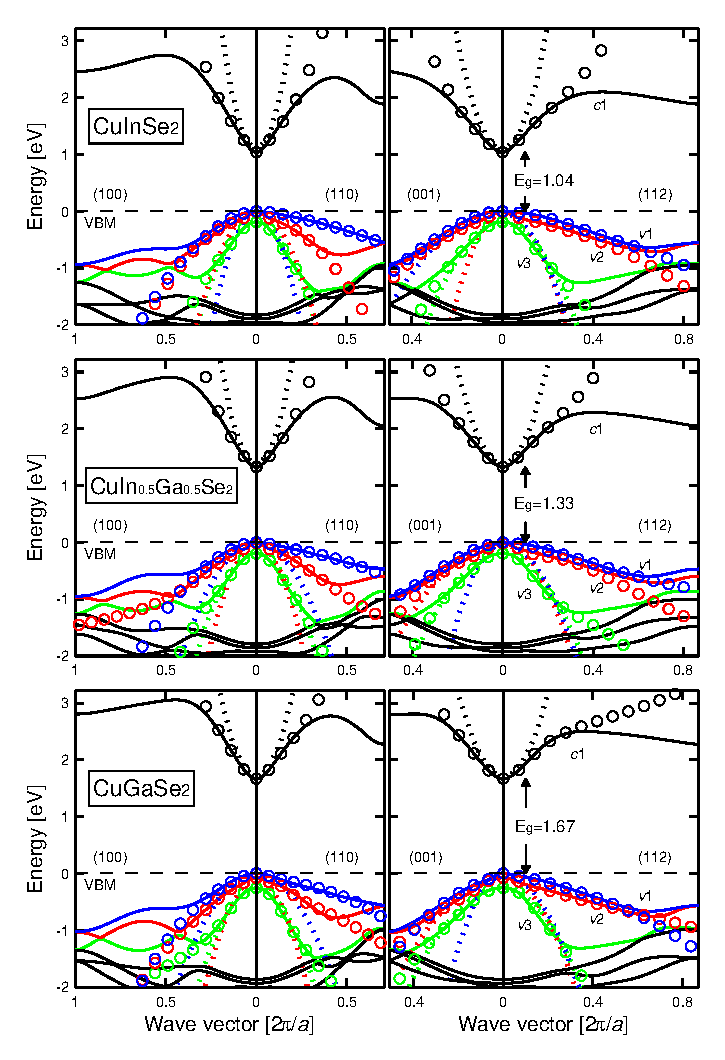
\includegraphics[width=0.95\textwidth]{seminar/bandstructure}
  \end{minipage}% 
  \begin{minipage}{0.5\textwidth}
    \caption{  Electronic band structure along four directions. the circles are the results of the full band parameterization (fbp), and the dotted lines represent the parabolic band approximation. }
  \end{minipage}
\end{figure}
\end{frame}


\begin{frame}
\MyLogo
\begin{figure}[H]
\centering
%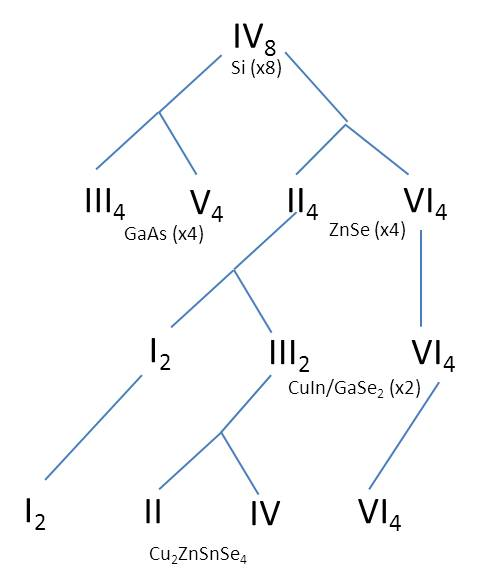
\includegraphics[scale=0.8]{compounds.jpg}
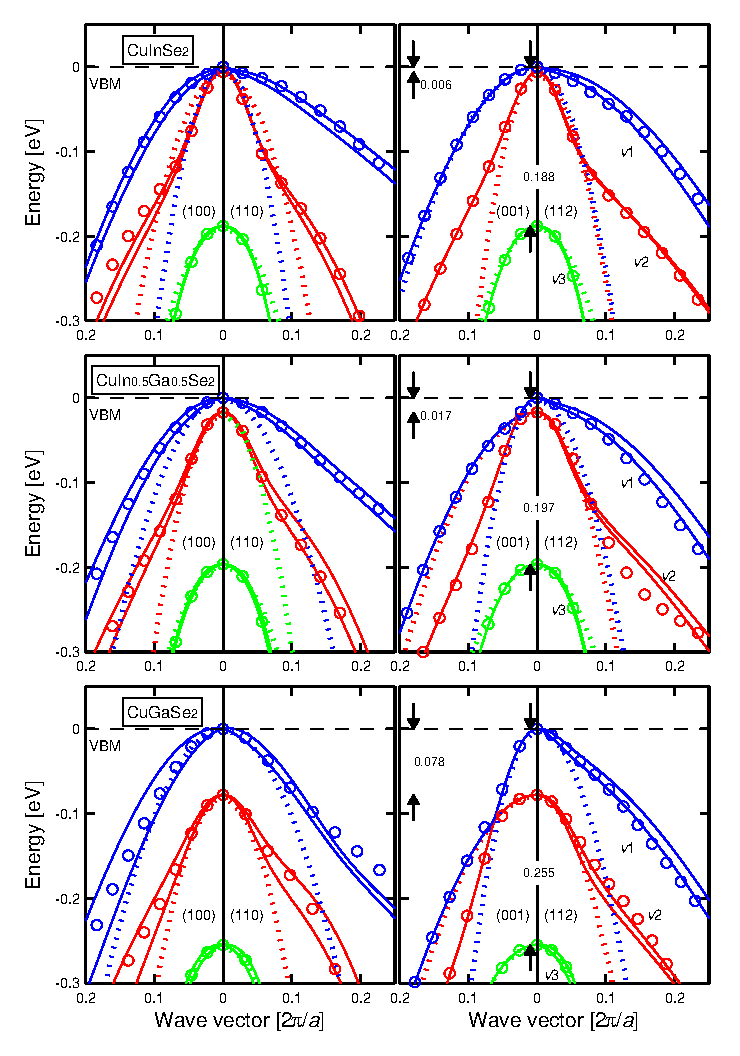
\includegraphics[width=0.42\textwidth,clip]{seminar/bandstructure_closeup} 
\caption{Close-up of above figure}
\label{closeup}
\end{figure}
\end{frame}

\begin{frame}
\MyLogo
\begin{figure}\label{dos}
  \begin{minipage}{0.5\textwidth} 
    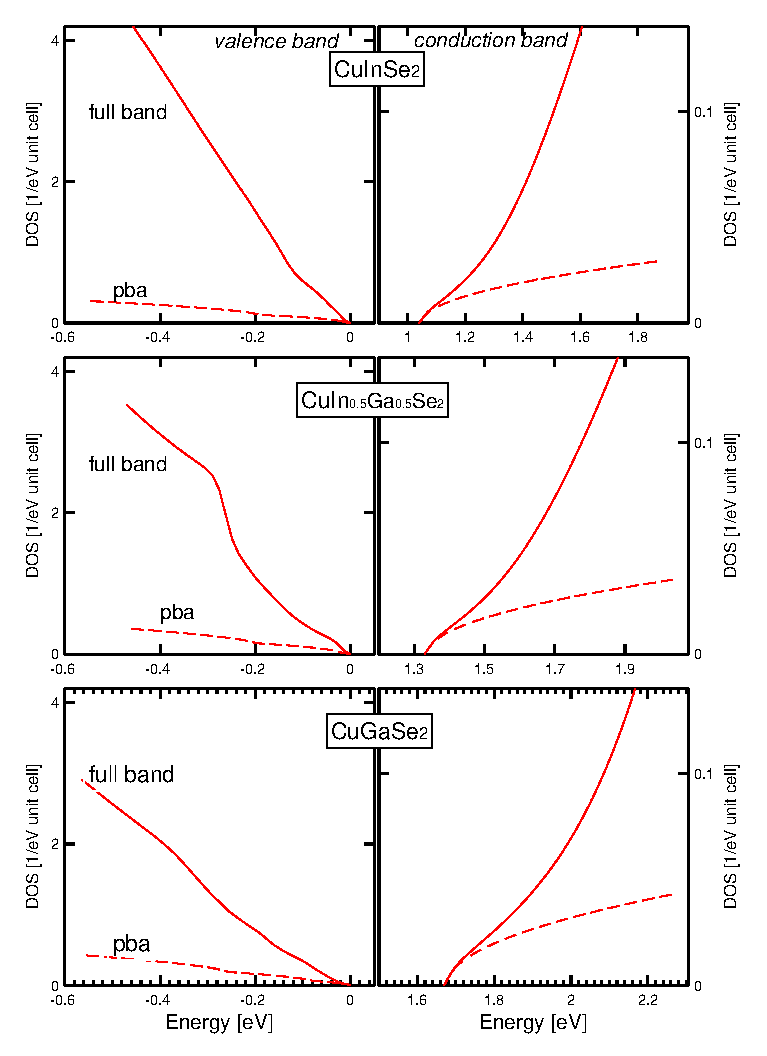
\includegraphics[width=0.95\textwidth]{seminar/dos}
  \end{minipage}% 
  \begin{minipage}{0.5\textwidth}
    \caption{  Total DOS ($ g_{v/c}(E)$) of the VBs (left panels) and of the CB (right panels) for $CuIn_{1-x}Ga_xSe_2$. The solid lines show the full band parameterization (fbp), and the dashed lines represent the parabolic band approximation (pba). }
  \end{minipage}
\end{figure}
\end{frame}


\begin{frame}
\MyLogo
\begin{figure}\label{dosmass}
  \begin{minipage}{0.5\textwidth} 
    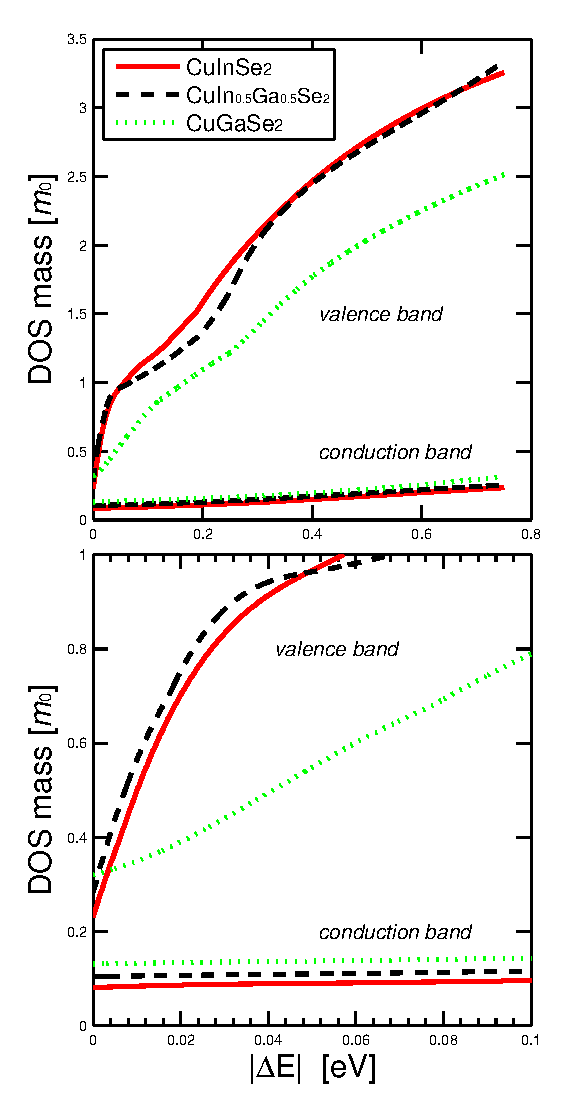
\includegraphics[width=0.7\textwidth]{seminar/dos_mass}
  \end{minipage}% 
  \begin{minipage}{0.5\textwidth}
    \caption{  The DOS mass of the VBs and the CB in $CuIn_{1-x}Ga_{x}Se_{2}$. The upper (lower) panel shows in a wider (narrower) energy region.}
  \end{minipage}
\end{figure}
\end{frame}




\begin{frame}
\MyLogo
\begin{figure}[H]
    \begin{center}
            \includegraphics[width=0.34\textwidth,clip]{seminar/fermi_sphere_cii}
            \includegraphics[width=0.3\textwidth,clip]{seminar/fermi_sphere_cig}
            \includegraphics[width=0.3\textwidth,clip]{seminar/fermi_sphere_cgg}
     \end{center}
    \caption{Constant energy surfaces for the three uppermost VBs and the lowest CB for the energies E = 1 meV (left column ellipsoidal) and E = 200 meV (right column). }
\end{figure}
\end{frame}




%\begin{frame}
%\MyLogo
%\begin{figure}\label{dosmass}
 % \begin{minipage}{0.5\textwidth} 
 %   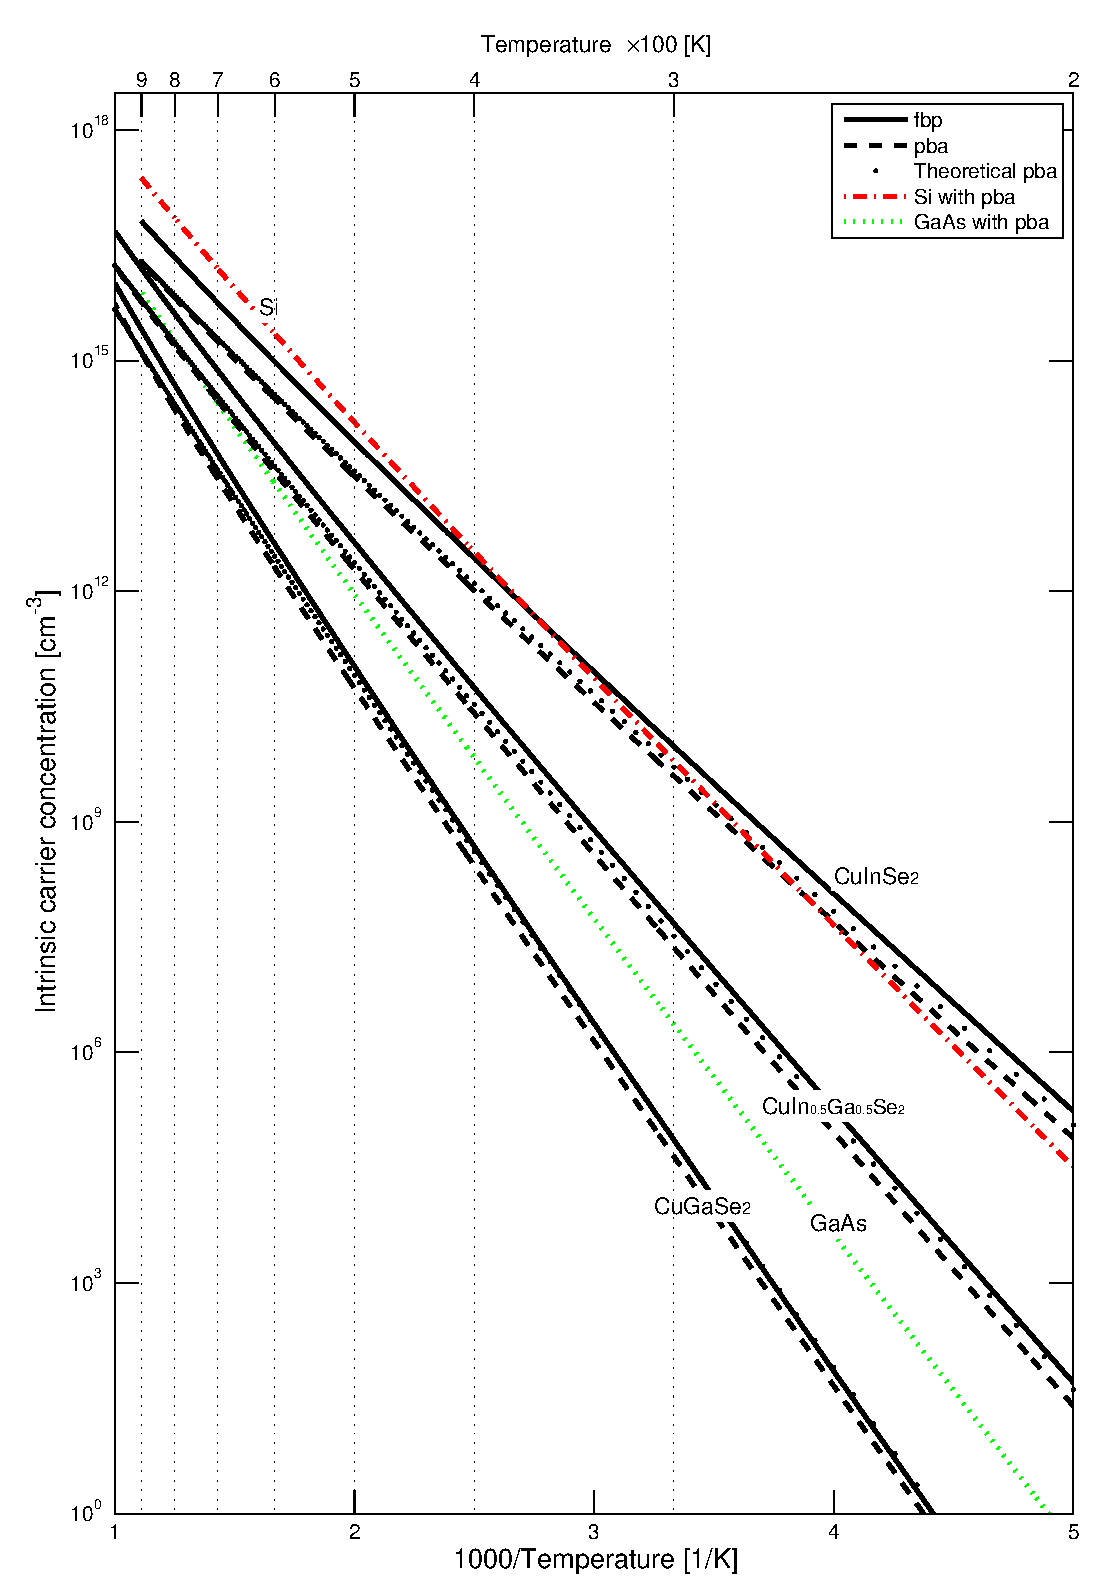
\includegraphics[width=0.9\textwidth]{seminar/intrinsic_carrier_concentration}
 % \end{minipage}% 
 % \begin{minipage}{0.5\textwidth}
 %   \caption{Intrinsic carrier concentration as function of temperature. For comparison, the theoretical result for GaAs and Si using the parabolic band approximation is given. }
 % \end{minipage}
%\end{figure}
%\end{frame}



\begin{frame}
\MyLogo
\begin{figure}[H]
    \begin{center}
            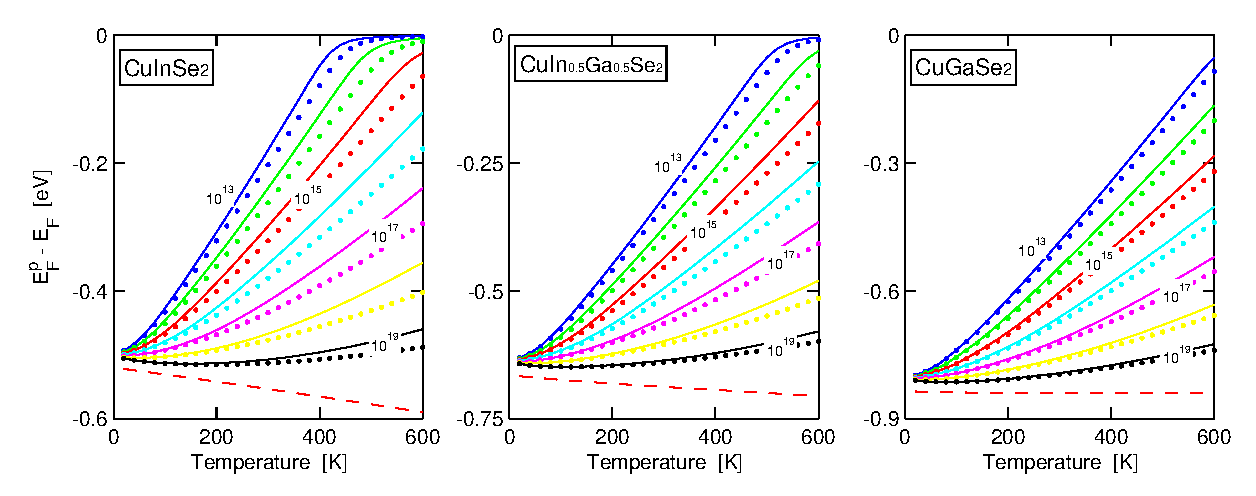
\includegraphics[width=1\textwidth,clip]{seminar/fermi_level_with_temperature}
     \end{center}
    \caption{Fermi level as functon of the temperature fo $p$-type $CuIn_{1-x}Ga_xSe_2$ for the effective doping concentration $N_A$ = $10^{13}, 10^{14}, 10^{15}, ... , $ and $10^{19}$ acceptors/$cm^3$. Solid and dotted lines represent the full band parameterization and the parabolic band approximation, respectively.}
\end{figure}
\end{frame}


\begin{frame}
\MyLogo
\begin{figure}[H]
    \begin{center}
            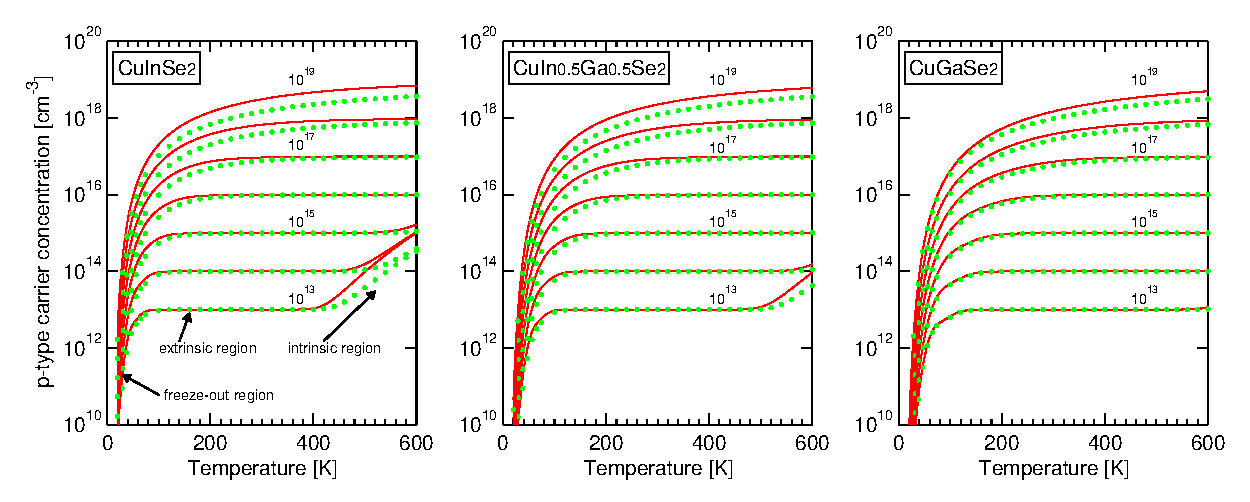
\includegraphics[width=1\textwidth,clip]{seminar/p_type_carrier_concentrication}
     \end{center}
    \caption{Free carrier concentration as function for the temperature in $p-type$ for the effective doping concentration $N_A$ = $10^{13}, 10^{14}, 10^{15}, ... , $ and $10^{19}$ acceptors/$cm^3$. Solid and dotted lines represent the full band parameterization and the parabolic band approximation, respectively.}
\end{figure}
\end{frame}


\section{Optical Properties of   $ {CuIn_{0.5}Ga_{0.5}Se_2} $}
\begin{frame}
\MyLogo

\raggedright {The dielectric function spectra of $CuIn_{0.5}Ga_{0.5}Se_{2}$ is calculated with full-potential linearized augmented plane wave method (Wien2k) using the generalized gradient approximation plus an onsite Coulomb interaction $U$ of the Cu $d$ states, it is compared with experiment as well. Probable electronic origins of the interband critical features (CPs) observed are discussed.}

\end{frame}


\begin{frame}
\MyLogo
\begin{figure}[H]
    \begin{center}
            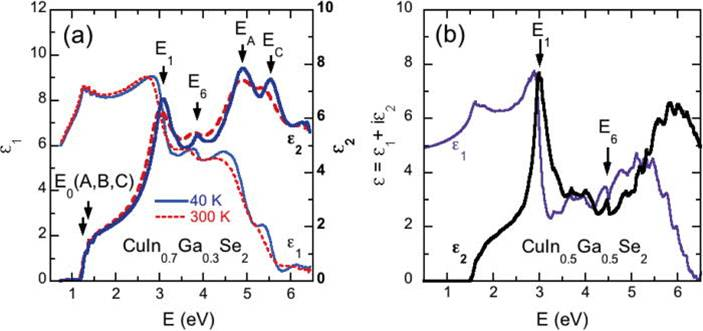
\includegraphics[width=1\textwidth,clip]{seminar/dielectric_function.jpg}
     \end{center}
    \caption{(a) Modeled dielectric function spectra for $CuIn_{0.7}Ga_{0.3}Se_2$ taken at 40 K and 300 K. The dielectric function for $CuIn_{0.5}Ga_{0.5}Se_{2}$ calculated by the FPLAPW using the GGA+U}
\end{figure}
\end{frame}

\begin{frame}
\MyLogo
\begin{figure}[H]
    \begin{center}
            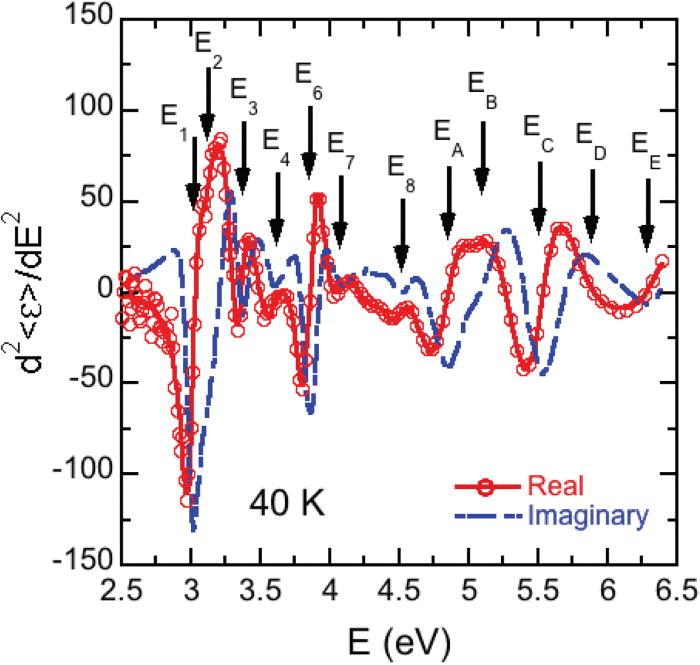
\includegraphics[width=0.5\textwidth,clip]{seminar/CP.jpg}
     \end{center}
    \caption{ Solid red are standard CP lineshapes bet fit to $d^2<\varepsilon_1>/dE^2$ (open circles) and dashed-dotted blue lines are  $d^2<\varepsilon_2>/dE^2$. Energies of each CP are indicated by arrows and labeled in a numeric and alphabetic order.}
\end{figure}
\end{frame}


\begin{frame}
\MyLogo
\begin{figure}[H]
    \begin{center}
            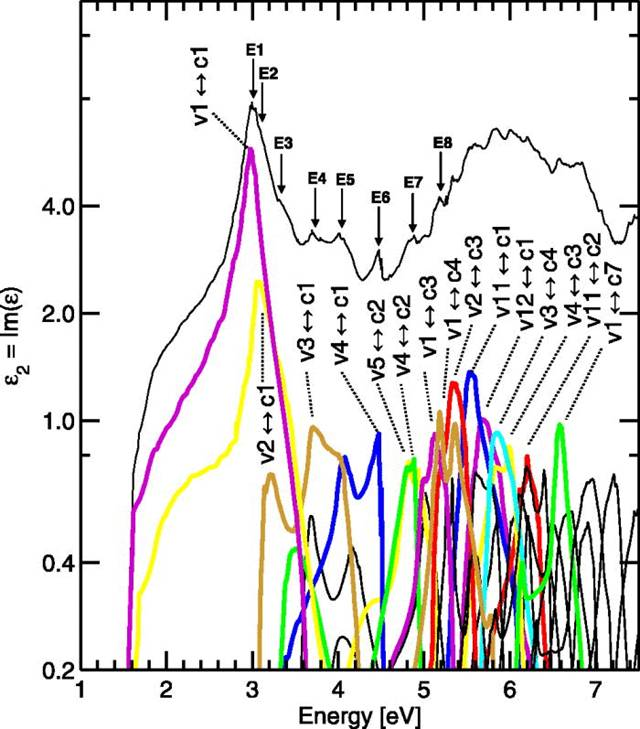
\includegraphics[width=0.5\textwidth,clip]{seminar/Band_to_band_analysis}
     \end{center}
    \caption{ Band-to-band analysis of the contribution to the total $\varepsilon_2$ spectrum. The most important valence-to-conduction band transitions are marked. Spin-orbit coupling is included.}
\end{figure}
\end{frame}


\begin{frame}
\MyLogo
\begin{figure}[H]
    \begin{center}
            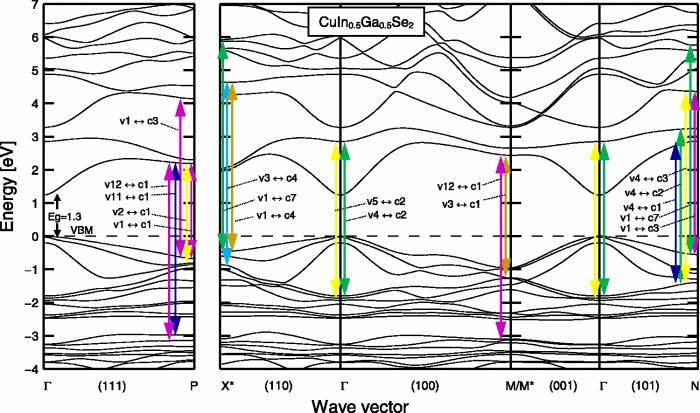
\includegraphics[width=1\textwidth,clip]{seminar/CPs}
     \end{center}
    \caption{The calculated electronic band structure of $CuIn_{0.5}Ga_{0.5}Se_2$ where the CPs are identified along the main sysmetry directions.}
\end{figure}
\end{frame}





\section{Current Work}
\begin{frame}
\MyLogo

\raggedright {I am involved in the implementation of the Exciting Code (Prof. Claudia Draxl), which is full-potential all-electron density-functional-theory (DFT) package implementing the families of linearized augmented planewave (LAPW) methods.
The main work is about scalar relativistic approximation, spin-orbit coupling and new $K \cdot P $ method. Everything is under development now.}

\vspace*{3\baselineskip}

The code mainpage is http://exciting-code.org/, which has many features (TDDFT, GW and BSE ...).

\end{frame}


\section{}
\begin{frame}
\MyLogo
\begin{center}
 \Huge Thank you for your time!
\end{center}
\end{frame}



\end{document}
